% As it was said before, \textit{MFCCs} are the acoustic features chosen for this work.
% Even though these raw features extracted from each frame composing the utterances of a phones
% would be enough to train a classifier that separates correctly
% pronounced and mispronounced phones, a different strategy can be taken. The features of all the
% frames of a particular utterance can be gathered together in order to summarize the
% general properties of the utterance. This is the purpose of using Legendre Polynomials when
% generating the features for the classifier. This technique has been used successfully
% in speaker recognition systems \cite{legendre}.

% \textit{Legendre functions} are the solutions to \textit{Legendre's differential equation}:

% \begin{equation}
% (1-x^{2})y''(x)-2xy'(x)+n(n+1)y(x)=0, \ for -1 \leq x \leq 1
% \end{equation}

% The solution for each particular $n={0, 1, 2 \dotsc} \in \mathbb{N}$ is a polynomial of degree
% $n$: $P_{n}(x)$. These solutions are well known for each $n \in \mathbb{N}$, and they can even
% be generated recursively. The first few Legendre Polynomials are:

% \begin{itemize}
%   \label{itemize:legendreTerms}
%   \item[] $P_{0}(x) = 1$
%   \item[] $P_{1}(x) = x$
%   \item[] $P_{2}(x) = \frac{1}{2}(3x^{2} - 1)$
%   \item[] $P_{3}(x) = \frac{1}{2}(5x^{3} - 3x)$
%   \item[] $P_{4}(x) = \frac{1}{8}(35x^{4} - 30x^{2} + 3)$
% \end{itemize}

% Legendre Polynomials are orthogonal with respect to the $L2 \ norm$ on the interval \mbox{$-1 \leq x \leq 1$}:

% \begin{equation}
% \int_{-1}^{1} P_{n}(x)*P_{m}(x)dx = 0, \ m \neq n
% \end{equation}

% Moreover, in the interval \mbox{$-1 \leq x \leq 1$} any function $f$ can be represented as sum of
% Legendre Polynomials, leading to the Fourier-Legendre Series:

% \begin{equation}
% f(x) = \sum_{0}^{\infty}a_{n}P_{n}(x)
% \end{equation}

% So an infinite terms of Legendre Polynomials over the interval \mbox{$-1 \leq x \leq 1$} can be used
% to approximate any function. Each coefficient models a particular aspect of the curve: $a_{0}$
% is interpreted as the \textit{mean} of the segment, $a_{1}$ is the slope, $a_{2}$ gives
% information about the curvature of the segment and the next coefficients model the fine details.
% A particular cutoff $c$ is chosen in order to limit the number of coefficients of the
% Legendre Polynomials to be picked in order to approximate the function in a reasonable manner
% while avoiding the complex details that may lead to overfitting.

% \subsection{Lasso Regression}

% Given the time instants $X=[x_{1}, x_{2} \dotsc x_{t}]$ and their respective values of a particular
% MFCC coefficient at those instants: $Y=[y_{1}, y_{2} \dotsc y_{t}]$,
% the problem of finding the coefficients of \textit{Legendre Polynomial} of degree $k$
% (for a previously defined $k$) that best approximates
% the values can be formulated in terms of a \textit{Least Squares} minimization problem:

% \begin{equation}
%   \min_{C} {\| AC - Y \|}^{2}
% \end{equation}

% where the solution of the system $C$ is a ($k+1$) vector that respresents the coefficients
% of the \textit{Legendre Polynomial} of degree $k$ that best approximates the points.
% $A$ is a $t$ x ($k$+1) matrix, where each column $i$ represents the result of computing
% \textit{Legendre's} $P_{i}$ polynomial (\ref{itemize:legendreTerms}) for each of the values
% $[x_{1}, x_{2}, \dotsc x_{t}]$, also known as the \textit{Legendre-Vandermonde} matrix:

% \begin{equation}
%   A =
%     \begin{pmatrix}
%       P_{0}(x_{1}) & P_{1}(x_{1}) & \cdots & P_{k}(x_{1}) \\
%       P_{0}(x_{2}) & P_{1}(x_{2}) & \cdots & P_{k}(x_{2}) \\
%       \vdots & \vdots & \ddots & \vdots \\
%       P_{0}(x_{t}) & P_{1}(x_{t}) & \cdots & P_{k}(x_{t}) \\
%     \end{pmatrix}
% \end{equation}

% When modeling a particular event is preferable to pick the simplest hypothesis that best
% explains the observations, because simpler hypothesis usually generalize better to new
% observations than more complex hypotheses. As it was said before, the higher the
% degree of the \textit{Legendre Polynomial},
% the more subtle details it models. In order to achieve the right balance between decreasing
% the least squares error and keeping the hypothesis simple two different measures are taken.
% On the one hand the degree of the polynomial $k$ is limited up to a few coefficients.
% On the other hand, a regularization technique of the \textit{Least Squares} family's
% problems is applied.

% The chosen regularization technique is called \textit{Lasso Regression}, and it modifies the
% original minimization problem by adding an additional term that penalizes the L1 norm of the
% solution:

% \begin{equation}
%   \min_{C} {\| AC - Y \|}^{2} + \lambda \| C \|_{1}
% \end{equation}

% Regularization terms leads to solutions where more responsibility is assigned to the
% coefficients that contributes the most in lowering the square errors of the error term while
% shrinking the coefficients with low contribution to the square error term.

% There exists other alternatives to \textit{Lasso} with regard to regularization.
% A widely-used one is \textit{Tikhonov Regularization}, also known as \textit{Ridge Regression},
% where the squared of the \textit{L2 norm:} $\| C \|_{2}^{2}$ is used as regularization term.

% In particular, the
% choice of using the \textit{L1 norm:} $\| C \|_{1}$ instead of the standard
% square of the \textit{L2 norm:} $\| C \|_{2}^{2}$ leads to an interesting and useful property.
% In \textit{Ridge Regression}, as the penalty is increased, all parameters are reduced while
% still remaining non-zero, while in \textit{Lasso} increasing the penalty will cause more and
% more of the parameters to be driven to zero. Thus \textit{Lasso} automatically selects more
% relevant features and discard the others whereas \textit{Ridge Regression} never fully
% discard any features.

% An intuitive explanation of why \textit{Lasso} behaves this way can be sketch out in terms
% of the shape of the sharped-edge region
% determined by the constraints of the regularization term.
% The level curves imposed by the least squares term will most likely hit the corners of
% that sharped-edge region, driving the values of some of the coefficients to zero.

% \begin{figure}[H]
%   \centering
%   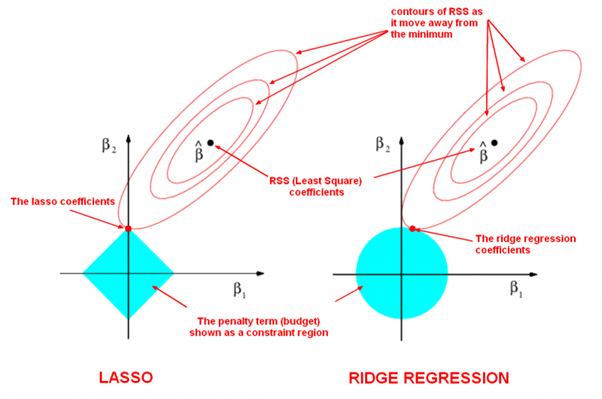
\includegraphics[width=0.5\textwidth]{files/figures/method/lasso-regression}
%   \caption{Intersection of the level curves of the \textit{Residual Sum of Squares}
%   \textit{RSS} with the regions imposed by the regularization terms. Unlike
%   \textit{Ridge Regression}, in \textit{Lasso Regression} the instersection is
%   most likely to happen at a corner of the sharped-edge region determined by the
%   \textit{L1-norm} regularization constraint, where the value of some of the coefficients
%   is equal to 0.}
% \end{figure}
